\chapter{Results}
\label{results}
Both optimization methods described in previous chapters should optimize code for the Bobox framework to some extent. This chapter covers performance evaluation of optimized and unoptimized code for both methods. However, each method is evaluated separately. There is a specific use case for each method, when it should stand out.

\section{Prefetch method}
\label{results-prefetch}
The goal of this optimization method is to reduce a number of short-running tasks. Specifically, tasks that are scheduled even though they do not have all input data for a meaningful execution. The gain in a speedup with this optimization method is the scheduling overhead. It only matters how often this situation occurs in user code.

In order to measure the scheduling overhead, it is necessary to maximize the number of wrongly scheduled tasks. A wrongly scheduled task has to have at least two inputs and there has to be some delay between getting data to its inputs. A bigger delay increases the possibility of the task being scheduled without all necessary data.

Furthermore, a parallel environment is not necessary in order to measure the scheduling overhead. It is harder to achieve the situation when a wrong scheduling matters with more logical threads. Wrong scheduling on free logical threads does not affect the overall performance. Thus, measurements are done on a single thread.

\subsection{Model}
There has to be a box with more than one input for the wrong scheduling and there can be more such boxes for a bigger effect. Now, it is necessary to create some mechanism to maximize the number of situations when a box is scheduled wrongly. This mechanism consist from a chain of boxes where each one creates input data for one specific input on all boxes that are supposed to be scheduled wrongly. All boxes from this chain, apart from the last box, then trigger scheduling of the next box in the chain that will create data for a different input on wrongly scheduled boxes.

Figure~\ref{prefetch-model} shows the model used in measurements. However, the number of distribution and collection boxes as well as the number of their inputs and outputs may vary. The figure shows only a \emph{pattern} used in the model construction. If all collection boxes prefetch only the first input or no input at all, the expected scheduling in the execution of a model instance constructed from the model in Figure~\ref{prefetch-model} is:

\begin{enumerate}
\item{control\_box}
\item{distribution\_box}
\item{Three times collection\_box - pop data from the first input and wait}
\item{distribution\_box}
\item{Three times collection\_box - pop data from the second input and wait}
\item{distribution\_box}
\item{Three times collection\_box - pop data from the last input and produce an output}
\item{sink\_box}
\end{enumerate}

\tikzset{model-node/.style={draw, rectangle, thick, rounded corners}}
\tikzset{model-path/.style={->, draw, thick}}
\tikzset{model-io/.style={draw, rectangle, thick, fill=black!75, inner sep=1.25pt}}

\begin{figure}[h!]
\caption{The model used in measurements of the prefetch method optimization with three distribution and three collection boxes.}
\label{prefetch-model}
\vspace{.5cm}
\centering
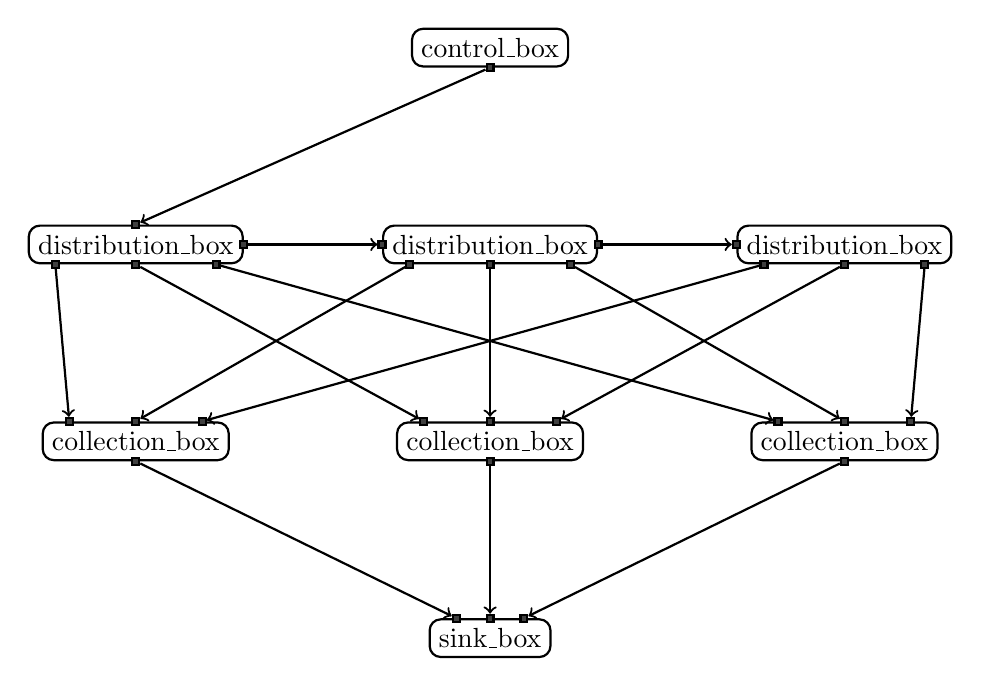
\begin{tikzpicture}[node distance=2.5cm]	
	% dist0 box
	\node[model-node](dist0){distribution\_box};
	\node[model-io](dist0in) at (dist0.north) {};
	\node[model-io](dist0outnext) at (dist0.east) {};
	\node[model-io, xshift=10pt](dist0out0) at (dist0.south west) {};
	\node[model-io](dist0out1) at (dist0.south) {};
	\node[model-io, xshift=-10pt](dist0out2) at (dist0.south east) {};
	
	% dist1 box
	\node[model-node, right of=dist0, xshift=2cm](dist1){distribution\_box};
	\node[model-io](dist1in) at (dist1.west) {};
	\node[model-io](dist1outnext) at (dist1.east) {};
	\node[model-io, xshift=10pt](dist1out0) at (dist1.south west) {};
	\node[model-io](dist1out1) at (dist1.south) {};
	\node[model-io, xshift=-10pt](dist1out2) at (dist1.south east) {};
	
	% dist2 box
	\node[model-node, right of=dist1, xshift=2cm](dist2){distribution\_box};
	\node[model-io](dist2in) at (dist2.west) {};
	\node[model-io, xshift=10pt](dist2out0) at (dist2.south west) {};
	\node[model-io](dist2out1) at (dist2.south) {};
	\node[model-io, xshift=-10pt](dist2out2) at (dist2.south east) {};
	
	% control box
	\node[model-node, above of=dist1](control){control\_box};
	\node[model-io](controlout) at (control.south) {};
	
	% control paths
	\path[model-path](controlout) -- (dist0in) {};
	\path[model-path](dist0outnext) -- (dist1in) {};
	\path[model-path](dist1outnext) -- (dist2in) {};
	
	% collection boxes
	\node[model-node, below of=dist0](coll0){collection\_box};
	\node[model-io, xshift=10pt](coll0in0) at (coll0.north west) {};
	\node[model-io](coll0in1) at (coll0.north) {};
	\node[model-io, xshift=-10pt](coll0in2) at (coll0.north east) {};
	\node[model-io](coll0out) at (coll0.south) {};
	\node[model-node, below of=dist1](coll1){collection\_box};
	\node[model-io, xshift=10pt](coll1in0) at (coll1.north west) {};
	\node[model-io](coll1in1) at (coll1.north) {};
	\node[model-io, xshift=-10pt](coll1in2) at (coll1.north east) {};
	\node[model-io](coll1out) at (coll1.south) {};
	\node[model-node, below of=dist2](coll2){collection\_box};
	\node[model-io, xshift=10pt](coll2in0) at (coll2.north west) {};
	\node[model-io](coll2in1) at (coll2.north) {};
	\node[model-io, xshift=-10pt](coll2in2) at (coll2.north east) {};
	\node[model-io](coll2out) at (coll2.south) {};
		
	% sink node	
	\node[model-node, below of=coll1](sink){sink\_box};
	\node[model-io, xshift=10pt](sinkin0) at (sink.north west) {};
	\node[model-io](sinkin1) at (sink.north) {};
	\node[model-io, xshift=-10pt](sinkin2) at (sink.north east) {};
	
	% collection paths
	\path[model-path](dist0out0) -- (coll0in0) {};
	\path[model-path](dist0out1) -- (coll1in0) {};
	\path[model-path](dist0out2) -- (coll2in0) {};
	\path[model-path](dist1out0) -- (coll0in1) {};
	\path[model-path](dist1out1) -- (coll1in1) {};
	\path[model-path](dist1out2) -- (coll2in1) {};
	\path[model-path](dist2out0) -- (coll0in2) {};
	\path[model-path](dist2out1) -- (coll1in2) {};
	\path[model-path](dist2out2) -- (coll2in2) {};
	
	% sink paths
	\path[model-path](coll0out) -- (sinkin0) {};
	\path[model-path](coll1out) -- (sinkin1) {};
	\path[model-path](coll2out) -- (sinkin2) {};
\end{tikzpicture}
\end{figure}

If all collection boxes prefetch their all input data, step 3 and step 5 are skipped. These prefetch calls can save up to six schedules when boxes do nothing meaningful.

\subsection{Benchmarks}
There are two boxes in the model without any description. The control box repeatedly produces data for distribution boxes. It yields each time after data is produced. The sink box is there for a debugging purpose. All boxes do minimal work apart from a communication with the Bobox framework to maximize the impact of the scheduling.

\begin{figure}[h!]
\vspace{.5cm}
\centering
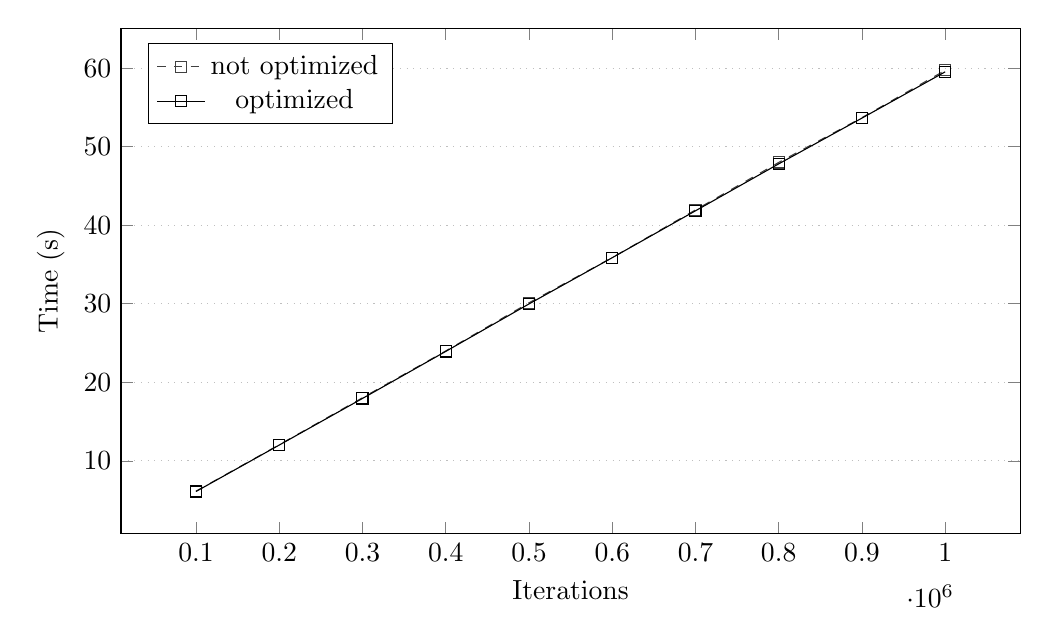
\begin{tikzpicture}
\begin{axis}[
	width=13cm,
	height=8cm,
	xlabel=Iterations,
	ylabel=Time (s),
	domain=100000:1000000,
	samples=12,
	legend pos=north west,
	ymajorgrids=true,
	grid style=dotted]

	% unoptimized code	
	\addplot[color=black!75, mark=square, mark options=solid, dashed]coordinates{
		(100000,6.133)
		(200000,12.041)
		(300000,18.026)
		(400000,23.984)
		(500000,30.111)
		(600000,35.871)
		(700000,41.939)
		(800000,47.991)
		(900000,53.692)
		(1000000,59.718)};
	\addlegendentry{not optimized}

	% optimized code
	\addplot[color=black, mark=square, solid, mark options=solid]coordinates{
		(100000,6.09)
		(200000,12.002)
		(300000,17.938)
		(400000,23.926)
		(500000,29.970)
		(600000,35.857)
		(700000,41.830)
		(800000,47.808)
		(900000,53.635)
		(1000000,59.528)};
	\addlegendentry{optimized}
\end{axis}
\end{tikzpicture}
\caption{Benchmarks for the prefetch optimization method with ten distribution and ten collection boxes.}
\label{prefetch-bench}
\end{figure}

Figure~\ref{prefetch-bench} shows results for the model with ten distribution and ten collection boxes. The dashed line shows times for not optimized code, the solid line shows times for  optimized code. X-axis represents the number of iterations in the control box. Y-axis represents execution times.

Even though the graph does not show it well, optimized code is very slightly faster in  most measurements. However, the gain in a speedup is negligible even for a bigger number of iterations or a bigger number of collection and distribution boxes. Furthermore, the gain in a speedup is approximately the same for a bigger number of iterations as for a lower number of iterations. The speedup appears to be constant for measured results. These results do not correspond with the expected behavior.

\subsection{Optimizer tweak}
It is necessary to look more into details of the presented model in Figure~\ref{prefetch-model} and the Bobox framework implementation to understand why there is a negligible speedup from unoptimized to optimized code. Both distribution and collection types of boxes are stateless. The Bobox framework allocates some objects of stateless boxes, initializes them by calling the \code{init\_impl} member function and reuses those allocated objects all over again. But, \code{init\_impl} is not called again when object is reused. Thus, prefetch calls added by this optimization method do not help anymore when the framework reuses boxes.

The prefetch optimization method is enhanced to add all prefetch calls for all used inputs to the end of the box execution member function body. This option is configurable and turned off by default. Figure~\ref{prefetch-bench-attach} shows results with this optimization tweak turned on compared to not optimized code. The improvement in a speedup is clearly visible.

\begin{figure}[h!]
\vspace{.5cm}
\centering
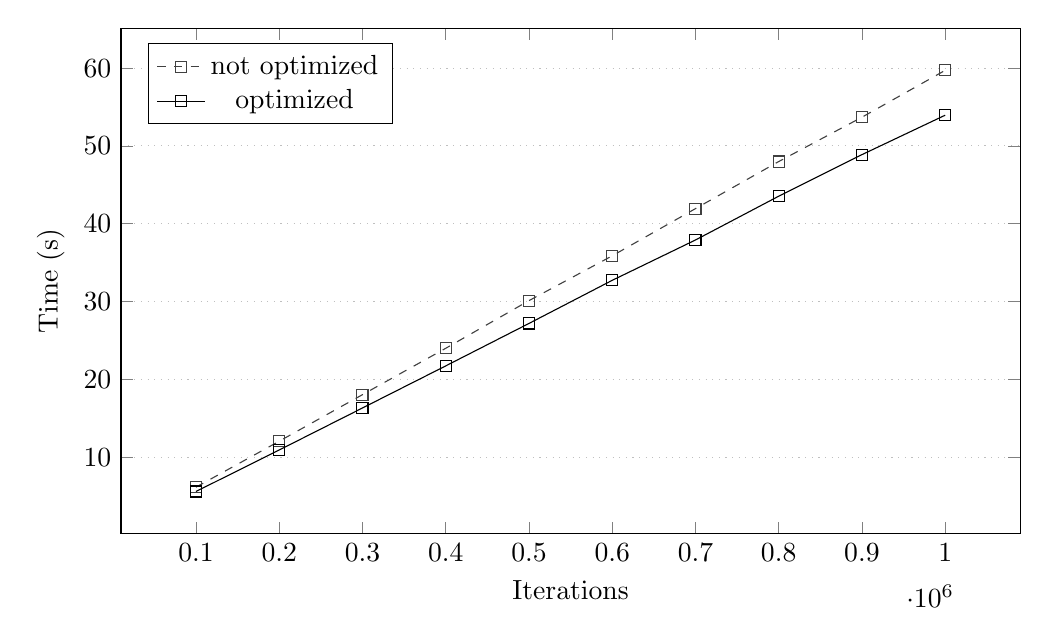
\begin{tikzpicture}
\begin{axis}[
	width=13cm,
	height=8cm,
	xlabel=Iterations,
	ylabel=Time (s),
	domain=100000:1000000,
	samples=12,
	legend pos=north west,
	ymajorgrids=true,
	grid style=dotted]

	% not optimized code	
	\addplot[color=black!75, mark=square, mark options=solid, dashed]coordinates{
		(100000,6.133)
		(200000,12.041)
		(300000,18.026)
		(400000,23.984)
		(500000,30.111)
		(600000,35.871)
		(700000,41.939)
		(800000,47.991)
		(900000,53.692)
		(1000000,59.718)};
	\addlegendentry{not optimized}

	% optimized code
	\addplot[color=black, mark=square, solid, mark options=solid]coordinates{
		(100000,5.58)
		(200000,10.912)
		(300000,16.313)
		(400000,21.722)
		(500000,27.180)
		(600000,32.722)
		(700000,37.907)
		(800000,43.537)
		(900000,48.880)
		(1000000,53.951)};
	\addlegendentry{optimized}
\end{axis}
\end{tikzpicture}
\caption{Benchmarks for the prefetch optimization method with ten distribution and ten collection boxes and the \textit{attach to execution body} tweak turned on.}
\label{prefetch-bench-attach}
\end{figure}

\subsection{Conclusion}
The Bobox scheduler is greatly optimized. Even in the presented scenario with approximately 10 boxes scheduled 9 times out of 10 wrongly, the speedup with 1 million iterations is only 5,767 seconds from 59,718 seconds to 53,951 seconds. Furthermore, tests were measured on a single logical thread. It is much harder to achieve this scenario with multiple logical threads. The scenario itself is artificial to showcase the optimization potential. On the other hand, there are software products where every second matters and there is no reason to turn off this optimization.

However, there is still one factor that is not tested well in the presented scenario, cache usage. Since all boxes do not work with data excessively, their cache usage is minimal. Most data can be probably held in cache the whole execution time. On the other hand, a scheduled box without all input data probably immediately reschedules. Thus, its impact on a cache is negligible anyway.

\section{Yield complex method}
The goal of this optimization method is to reduce a number of long-running tasks. Such tasks can inhibit a parallel execution, thus vastly increase execution times. On the other hand, long-running tasks are more cache friendly, but the speedup from a parallelism should be much bigger than the one from a better cache usage.

\subsection{Model}
Measurements are done on a model with one important task. This task is essential for a parallel execution and it should run as often as possible. But, there are also long-running tasks which prevent scheduling of this essential task, thus they inhibit parallelism.

Figure~\ref{yield-model} shows an example of a model with one important task. The source box is a box that computes data for a parallel processing and distributes this data to worker boxes. Worker boxes process data in parallel. If there is the same number of worker boxes as the number of logical threads, there is a big possibility that the scheduler immediately schedules all worker boxes to all logical threads. The worker box is the long-running task. Thus, all worker boxes keep the source box out of an execution. This source box creates the bottleneck for a parallel execution.

\begin{figure}[h!]
\vspace{.5cm}
\centering
\caption{The model used in measurements of the yield optimization method with four logical threads.}
\label{yield-model}
\begin{tikzpicture}[node distance=3cm]	
	% worker0
	\node[model-node, minimum height=4cm](worker0){worker\_box};
	\node[model-io](worker0in) at (worker0.north) {};
	\node[model-node, yshift=-0.9cm, minimum width=2cm, minimum height=1.35cm](worker0task0) at (worker0.north) {work};
	\node[model-node, yshift=0.9cm, minimum width=2cm, minimum height=1.35cm](worker0task1) at (worker0.south) {work};
	
	% worker1
	\node[model-node, minimum height=4cm, right of=worker0](worker1){worker\_box};
	\node[model-io](worker1in) at (worker1.north) {};
	\node[model-node, yshift=-0.9cm, minimum width=2cm, minimum height=1.35cm](worker1task0) at (worker1.north) {work};
	\node[model-node, yshift=0.9cm, minimum width=2cm, minimum height=1.35cm](worker1task1) at (worker1.south) {work};
	
	% worker2
	\node[model-node, minimum height=4cm, right of=worker1](worker2){worker\_box};
	\node[model-io](worker2in) at (worker2.north) {};
	\node[model-node, yshift=-0.9cm, minimum width=2cm, minimum height=1.35cm](worker2task0) at (worker2.north) {work};
	\node[model-node, yshift=0.9cm, minimum width=2cm, minimum height=1.35cm](worker2task1) at (worker2.south) {work};
	
	% worker3
	\node[model-node, minimum height=4cm, right of=worker2](worker3){worker\_box};
	\node[model-io](worker3in) at (worker3.north) {};
	\node[model-node, yshift=-0.9cm, minimum width=2cm, minimum height=1.35cm](worker3task0) at (worker3.north) {work};
	\node[model-node, yshift=0.9cm, minimum width=2cm, minimum height=1.35cm](worker3task1) at (worker3.south) {work};
	
	% source box
	\node(middle) at ($(worker1)!0.5!(worker2)$){};
	\node[model-node, minimum width=2cm, minimum height=1.35cm, above of=middle, yshift=1cm](source){source\_box};
	\node[model-io](sourceout) at (source.south){};
	
	% paths
	\path[model-path](sourceout) -- (worker0in){};
	\path[model-path](sourceout) -- (worker1in){};
	\path[model-path](sourceout) -- (worker2in){};
	\path[model-path](sourceout) -- (worker3in){};
	
\end{tikzpicture}
\end{figure}

If worker boxes finish approximately at the same time, the source box is scheduled and until it finishes, nothing runs in parallel. But, if one worker box yields its execution and let the source box to run, data for the next bunch of parallel worker boxes is ready sooner. Even thought the particular worker box ends later, it does not inhibit parallelism as there are always data for other workers. A bigger task granularity greatly helps in this particular model example.

\subsection{Benchmarks}
Measurements were done on a parallel environment with eight logical threads. Therefore, the model consists of eight stateless worker boxes and single source box. The worker box \textit{calculates} for ten seconds and the source box \textit{calculates} for five seconds. There would be different overall times measured for different times of a boxes execution, but the ratio between optimized and unoptimized code is expected to be the same. This optimization method causes the worker box to yield after five seconds. Figure~\ref{yield-bench} shows measured results.

But, measured results in Figure~\ref{yield-bench} are a bit different from the expected outcome. If the source box is the bottleneck of an execution, it should inhibit the parallel execution for five seconds each iteration. So the speedup for ten iterations should be approximately fifty seconds. The measured result is approximately twenty seconds.

\begin{figure}[h!]
\vspace{.5cm}
\centering
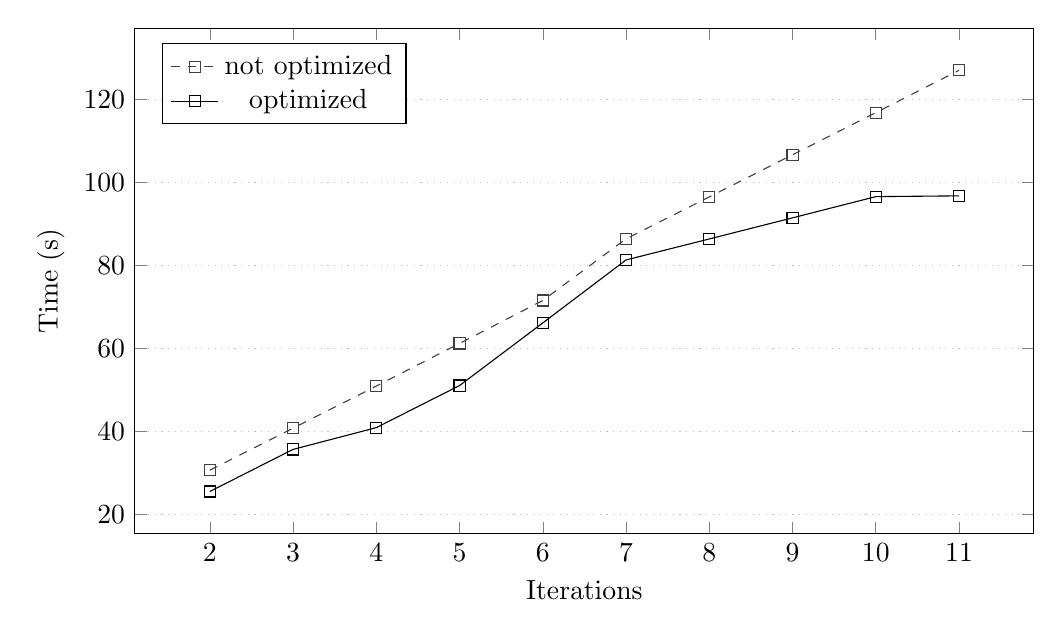
\begin{tikzpicture}
\begin{axis}[
	width=13cm,
	height=8cm,
	xlabel=Iterations,
	ylabel=Time (s),
	domain=2:11,
	samples=12,
	legend pos=north west,
	ymajorgrids=true,
	grid style=dotted]

	% unoptimized code	
	\addplot[color=black!75, mark=square, mark options=solid, dashed]coordinates{
		(2,30.730)
		(3,40.846)
		(4,50.996)
		(5,61.268)
		(6,71.616)
		(7,86.476)
		(8,96.565)
		(9,106.726)
		(10,116.863)
		(11,127.066)};
	\addlegendentry{not optimized}

	% optimized code
	\addplot[color=black, mark=square, solid, mark options=solid]coordinates{
		(2,25.597)
		(3,35.736)
		(4,40.980)
		(5,51.121)
		(6,66.206)
		(7,81.380)
		(8,86.444)
		(9,91.526)
		(10,96.637)
		(11,96.826)};
	\addlegendentry{optimized}
\end{axis}
\end{tikzpicture}
\caption{Benchmarks for the yield optimization method with eight logical threads and eight worker boxes, the naive implementation.}
\label{yield-bench}
\end{figure}

The problem is the implementation of the source box for these particular measurements. The source box calculates something for five seconds, then it sends envelopes to all worker boxes and it yields immediately. But, the Bobox scheduler does not schedule all worker boxes immediately after the source box yields. The source box is often scheduled with the bunch of worker boxes and delays an execution of one of them. However, there is still a significant speedup in the execution.

The source box has to do some additional work before it yields to achieve the described behavior. It gives time to the Bobox scheduler to schedule seven worker boxes and the yield in the source box schedules the last worker box. Figure~\ref{yield-bench-better} shows measured results with this described implementation and the speedup approximately matches expected numbers.

\begin{figure}[h!]
\vspace{.5cm}
\centering
\caption{Benchmarks for the yield optimization method with eight logical threads and eight worker boxes.}
\label{yield-bench-better}
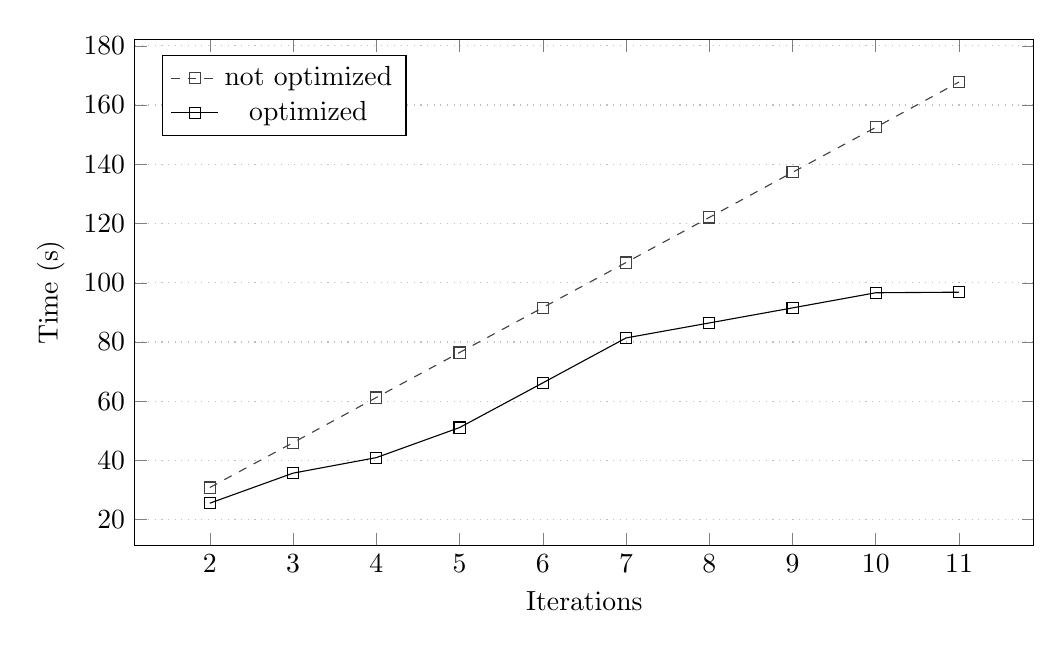
\begin{tikzpicture}
\begin{axis}[
	width=13cm,
	height=8cm,
	xlabel=Iterations,
	ylabel=Time (s),
	domain=2:11,
	samples=12,
	legend pos=north west,
	ymajorgrids=true,
	grid style=dotted]

	% unoptimized code	
	\addplot[color=black!75, mark=square, mark options=solid, dashed]coordinates{
		(2,30.881)
		(3,46.013)
		(4,61.263)
		(5,76.451)
		(6,91.616)
		(7,106.841)
		(8,122.057)
		(9,137.280)
		(10,152.462)
		(11,167.769)};
	\addlegendentry{not optimized}

	% optimized code
	\addplot[color=black, mark=square, solid, mark options=solid]coordinates{
		(2,25.597)
		(3,35.736)
		(4,40.980)
		(5,51.121)
		(6,66.206)
		(7,81.380)
		(8,86.444)
		(9,91.526)
		(10,96.637)
		(11,96.826)};
	\addlegendentry{optimized}
\end{axis}
\end{tikzpicture}
\end{figure}

\subsection{Conclusion}
The presented model lacks a good parallel design in the first place and a more skilled programmer would not probably write such code. But, this model can be \textit{hidden} in more complex models.

Long-running tasks can occur in a longer development process, when programmers extend a task to do more and more work with increasing requirements for application features. There may be various reasons such as a lack of time or even laziness to write code directly to an existing task. A programmer can also develop a long-running task because the work done by this task is monolithic and it is natural to write such code in a single function. This programmer may not realize consequences of such code to parallelism and forget to yield its execution. There are multiple ways how long-running tasks can occur in a code. This paragraph mentions only some of them.

The bigger granularity can greatly speedup an application execution. Furthermore, results of the prefetch optimization method show that even excessively short-running tasks that run excessively often affect execution times only very little. This optimization method can definitely speedup an application with very low risks.